\documentclass[a4paper,12pt,obeyspaces,spaces,hyphens]{article}

\def \trainingtitle{Développement de systèmes Linux embarqué}
\def \trainingduration{Formation sur site, 4 jours}

\usepackage{agenda}

\begin{document}

\feshowtitle

\small

\arrayrulecolor{lightgray} {
  \setlist[1]{itemsep=-5pt}
  \begin{tabularx}{\textwidth}{|g|h|}
    {\bf Titre} & {\bf Formation au développement de systèmes Linux embarqué} \\
    \hline

    {\bf Aperçu} &
Chaînes de compilation croisée, bibliothèques standard C pour l'embarqué. \par
Chargeurs de démarrage (bootloaders). \par
Configuration. compilation et démarrage du noyau Linux. \par
Applications et bibliothèques légères pour systèmes embarqués \par
Systèmes de fichiers pour stockage de type bloc \par
Outils de développement de systèmes embarqués Linux. \par
Développement et mise au point d'applications sur le système embarqué. \par
Travaux pratiques sur carte ARM STM32MP157D-DK1 Discovery Board. \\
    \hline
    {\bf Supports} &
    Vérifiez que le contenu de la formation correspond à vos besoins :
    \newline \url{https://bootlin.com/doc/training/embedded-linux}. \\
    \hline

    {\bf Durée} & {\bf Quatre} jours - 32 h (8 h par jour)
    \newline 50\% de présentations et 50\% de travaux pratiques. \\
    \hline

    {\bf Formateur} & Un des ingénieurs mentionnés sur :
    \newline \url{https://bootlin.com/training/trainers/}\\
    \hline

    {\bf Langue} & Présentations : Français
    \newline Supports : Anglais\\
    \hline

    {\bf Public ciblé} & Ingénieurs développant des systèmes embarqués
    reposant sur Linux et des composants open-source.\\
    \hline

    {\bf Pré-requis} &

    {\bf Connaissance et pratique des commandes UNIX ou
    GNU/Linux}
    \newline Les personnes n'ayant pas ces connaissances doivent
    s'autoformer, par exemple en utilisant nos supports de formation
    disponibles en ligne :
    \newline \url{https://bootlin.com/blog/command-line/} \vspace{1em}
    \\
    \hline

    {\bf Variante} & Version complète de la formation au développement
    de systèmes Linux embarqué, ({\bf durée de 5 jours}) avec 2
    demi-journées supplémentaires :
    \begin{itemize}
    \item Gestion de stockage de type flash et systèmes de fichiers
          spécialisés
    \item Implémentation de contraintes temps-réel avec Linux
    \end{itemize}
    \url{https://bootlin.com/doc/training/embedded-linux/embedded-linux-agenda-fr.pdf}.  \\
    \hline
  \end{tabularx}

  \begin{tabularx}{\textwidth}{|g|h|}
    {\bf Équipement\newline nécessaire} &
    {\bf Pour les sessions sur site uniquement}
    \newline Le matériel est fourni par Bootlin durant les
    sessions inter-entreprises
    \begin{itemize}
    \item Projecteur vidéo
    \item Un ordinateur sur chaque bureau (pour une ou deux personnes), avec au
    moins 8 Go de RAM et Ubuntu Linux installé dans une {\bf partition
    dédiée d'au moins 30 Go. L'utilisation de Linux dans une machine virtuelle
    n'est pas supportée}, en raison de problèmes avec la connexion au matériel.
    \item Nous avons besoin d'Ubuntu Desktop 20.04 (Xubuntu et autres
    variantes fonctionnent également). Nous ne supportons pas d'autres
    distributions, car nous ne pouvons tester toutes les versions des
    paquets.
    \item {\bf Connexion à Internet} (directe ou par le proxy de l'entreprise).
    \item {\bf Les ordinateurs contenant des données importantes doivent être
    sauvegardés} avant d'être utilisés dans nos sessions. Certains
    participants ont déjà commis des erreurs lors de travaux pratiques
    avec pour conséquence des pertes de données.
    \end{itemize} \\
    \hline

    {\bf Supports} & Copie électronique des présentations et travaux pratiques.
    \newline Version électronique des données pour les travaux
    pratiques..\\
    \hline

\end{tabularx}}
\normalsize

\feagendatwocolumn
{Matériel}
{
  La plateforme matérielle utilisée pendant les travaux pratiques de
  cette formation est la carte {\em STM32MP157D-DK1 Discovery de
    STMicroelectronics}, dont voici les caractéristiques :

  \begin{itemize}
  \item Processeur STM32MP157D avec deux coeurs ARM Cortex-A7
  \item Alimentation par USB-C powered
  \item 512 Mo de RAM DDR3L
  \item Port gigabit Ethernet
  \item 4 ports USB hôte 2.0
  \item 1 port USB-C OTG
  \item 1 connecteur micro SD
  \item Debugger ST-LINK/V2-1 intégré à la carte
  \item Broches compatibles Arduino Uno v3
  \item Codec audio
  \item Divers: boutons, LEDs
  \end{itemize}
}
{}
{
  \begin{center}
    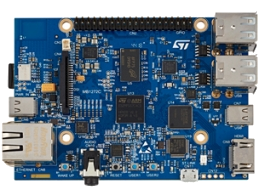
\includegraphics[height=5cm]{../slides/discovery-board-dk1/discovery-board-dk1.png}
  \end{center}
}

\section{1\textsuperscript{er} jour - Matin}

\feagendaonecolumn
{Cours – Introduction à Linux embarqué}
{
  \begin{itemize}
  \item Avantages de Linux par rapport aux autres OS pour l'embarqué.
	Raisons pour choisir Linux.
  \item Aperçu général : comprendre l'architecture d'un système Linux
	embarqué. Aperçu des principaux éléments dans un système typique.
  \end{itemize}
  {\em Le reste de la formation étudie chacun de ces éléments en détail.}
}
\\
\feagendatwocolumn
{Cours - Environnement de développement}
{
  \begin{itemize}
  \item Système d'exploitation et outils sur la station de travail
	pour le développement de systèmes Linux embarqué.
  \item Astuces pour l'utilisation de Linux sur station de travail.
  \end{itemize}
}
{Cours - Chaîne de compilation croisée et bibliothèque standard C}
{
  \begin{itemize}
  \item Les composants d'une chaîne de compilation croisée.
  \item Choisir une bibliothèque standard C.
  \item Le contenu de la bibliothèque standard C.
  \item Les chaînes de compilation croisée prêtes à l'emploi.
  \item La construction automatisée d'une chaîne de compilation croisée.
  \end{itemize}
}

\section{1\textsuperscript{er} Jour - Après-midi}
\feagendatwocolumn
{TP – Chaîne de compilation croisée}
{
  \begin{itemize}
  \item Configuration de Crosstool-NG
  \item Exécution pour construire une chaîne de compilation croisée
	personnalisée reposant sur la uClibc.
  \end{itemize}
}
{Cours – Chargeurs de démarrage}
{
  \begin{itemize}
  \item Chargeurs de démarrage existants
  \item Fonctionnalités des chargeurs de démarrage
  \item Installation d'un chargeur de démarrage
  \item Focus sur U-Boot
  \end{itemize}
}
\\

\feagendatwocolumn
{TP - U-Boot}
{
  {\em En utilisant la carte STM32MP157D-DK1}
  \begin{itemize}
  \item Mise en place de la communication série avec la carte.
  \item Configuration, compilation et installation du chargeur de
	démarrage de premier niveau et d'U-Boot sur la carte Discovery.
  \item Familiarisation avec l'environnement et les commandes d'U-Boot.
  \item Mise en place de la communication TFTP avec la carte.
	Utilisation des commandes TFTP d'U-Boot.
  \end{itemize}
}
{Cours – Noyau Linux}
{
  \begin{itemize}
  \item Rôle et architecture générale du noyau Linux.
  \item Fonctionnalités disponibles dans le noyau Linux, en insistant
	sur les fonctionnalités utiles dans les systèmes embarqués.
  \item L'interface entre le noyau et les applications.
  \item Récupérer les sources.
  \item Comprendre les versions du noyau.
  \item Utilisation de la commande patch.
  \end{itemize}
}
\\

\section{2\textsuperscript{ème} jour - Matin}

\feagendatwocolumn
{TP - Sources du noyau}
{
  \begin{itemize}
  \item Téléchargement des sources
  \item Application de patches
  \end{itemize}
}
{Cours – Configuration et compilation du noyau Linux}
{
  \begin{itemize}
  \item Configuration du noyau.
  \item Utilisation de configurations prêtes à l'emploi pour des cartes embarquées.
  \item Compilation du noyau.
  \item Fichiers générés à l'issue de la compilation.
  \item Utilisation des modules noyau.
  \end{itemize}
}

\feagendaonecolumn
{TP - Compilation croisée du noyau et démarrage sur la carte}
{
  {\em En utilisant la carte STM32MP157D-DK1}
  \begin{itemize}
  \item Configuration du noyau Linux et compilation croisée pour la carte ARM.
  \item Mise en place d'un serveur TFTP sur la station de développement.
  \item Téléchargement du noyau en utilisant le client TFTP d'U-Boot.
  \item Démarrage du noyau depuis la RAM.
  \item Copie du noyau vers la flash et démarrage depuis la flash.
  \item Stockage des paramètres de démarrage en flash et automatisation
	du démarrage du noyau.
  \end{itemize}
}

\section{2\textsuperscript{ème} jour - Après-midi}

\feagendatwocolumn
{Cours – Système de fichier racine}
{
  \begin{itemize}
  \item Les systèmes de fichiers dans Linux.
  \item Rôle et organisation du système de fichiers racine.
  \item Localisation de ce système de fichiers: sur espace
	de stockage, en mémoire, sur le réseau.
  \item Les fichiers device, les systèmes de fichiers virtuels.
  \item Contenu type d'un système de fichiers.
  \end{itemize}
}
{Cours - BusyBox}
{
  \begin{itemize}
  \item Présentation de BusyBox. Intérêt pour les systèmes embarqués.
  \item CConfiguration, compilation et installation.
  \end{itemize}
}

\feagendaonecolumn
{TP – Construction d'un minuscule système Linux embarqué avec BusyBox}
{
  {\em En utilisant la carte STM32MP157D-DK1}
  \begin{itemize}
  \item Construction à partir de zéro d'un système de fichiers racine
	contenant un système Linux embarqué
  \item Mise en place d'un noyau permettant de démarrer le système
	depuis un répertoire mis à disposition par la station de
	développement au travers de NFS.
  \item Passage de paramètres au noyau pour le démarrage avec NFS.
  \item Création complète du système de fichiers à partir de zéro :
	installation de BusyBox, création des fichiers spéciaux
	pour les périphériques.
  \item Initialisation du système en utilisant le programme init de BusyBox.
  \item Utilisation du serveur HTTP de BusyBox.
  \item Contrôle de la cible à partir d'un navigateur Web sur la
	station de développement.
  \item Mise en place des bibliothèques partagées sur la cible et
	développement d'une application d'exemple.
  \end{itemize}
}

\section{3\textsuperscript{ème} jour - Matin}

\feagendatwocolumn
{Cours - Système de fichiers bloc}
{
  \begin{itemize}
  \item Systèmes de fichiers pour périphériques bloc.
  \item Utilité des systèmes de fichiers journalisés.
  \item Systèmes de fichiers en lecture seule.
  \item Systèmes de fichiers en RAM.
  \item Création de chacun de ces systèmes de fichiers.
  \item Suggestions pour les systèmes embarqués.
  \end{itemize}
}
{TP - Système de fichiers bloc}
{
  {\em En utilisant la carte STM32MP157D-DK1}
  \begin{itemize}
  \item Créer des partitions sur le stockage bloc.
  \item Démarrage d'un système avec un assemblage de plusieurs systèmes
	de fichiers : SquashFS pour les applications, ext3 pour la
 	configuration et les données utilisateur et tmpfs pour les
	fichiers temporaires.
  \end{itemize}
}

\section{3\textsuperscript{ème} jour - Après-midi}

\feagendaonecolumn
{Cours – Réutilisation de composants open-source existants pour le système
embarqué}
{
  \begin{itemize}
  \item Motivations pour la réutilisation de composants existants.
  \item Trouver et choisir des composants libres et open-source existants.
  \item Les licences de Logiciels Libres et leurs conditions.
  \item Aperçu de composants typiquement utilisés dans les systèmes
	Linux embarqués : bibliothèques et systèmes graphiques (framebuffer,
	GTK, Qt, etc.), utilitaires système, bibliothèques et
	utilitaires réseau, bibliothèques multimédia, etc.
  \item Construction du système et intégration des composants.
  \end{itemize}
}

\feagendatwocolumn
{Cours – Compilation croisée de bibliothèques et d'applications}
{
  \begin{itemize}
  \item Configuration, compilation croisée et installation de bibliothèques
	et d'applications pour un système embarqué
  \item Détails sur le système de compilation utilisé dans la plupart
	des composants open-source.
  \item Aperçu des principaux problèmes rencontrés lors de la
	réutilisation des composants.
  \end{itemize}
}
{TP – Compilation croisée de bibliothèques et d'applications.}
{
  {\em Si suffisamment de temps disponible}
  \begin{itemize}
  \item Construction d'un système avec les bibliothèques ALSA et une
	application de lecture audio.
  \item Compilation et installation manuelle de plusieurs
	composants open-source.
  \item Apprentissage des principales techniques et des problèmes principaux.
  \end{itemize}
}

\section{4\textsuperscript{ème} jour - Matin}

\feagendatwocolumn
{Cours - Outils de construction de systèmes}
{
  \begin{itemize}
  \item Outils de la communauté pour la construction
	automatisée de systèmes.
  \item Exemple de Buildroot.
  \end{itemize}
}
{TP - Construction d'un système avec Buildroot}
{
  {\em En utilisant la carte STM32MP157D-DK1}
  \begin{itemize}
  \item Utilisation de Buildroot pour construire de façon automatisée
	un système similaire à celui du TP précédent.
  \item Voir à quel point cela est plus simple
  \item Optionnel: rajout d'un paquet dans Buildroot
  \end{itemize}
}

\section{4\textsuperscript{ème} jour - Après-midi}

\feagendaonecolumn
{Cours - Développement et déboguage d'application}
{
  \begin{itemize}
  \item Langages de programmations et bibliothèques disponibles.
  \item Aperçu de la bibliothèque C pour le développement d'applications.
  \item Systèmes de construction pour votre application, comment utiliser des
	bibliothèques existantes dans votre application.
  \item Environnements de développement intégrés (IDE) et lecteur de code source.
  \item Débogueurs : déboguage d'applications à distance avec gdb et gdbserver, analyse
	post-mortem d'une application.
  \item Analyseurs de code, analyseurs mémoire, outils de profiling.
  \end{itemize}
}

\feagendaonecolumn
{TP – Développement et déboguage d'application}
{
  {\em En utilisant la carte STM32MP157D-DK1}
  \begin{itemize}
  \item Développement et compilation d'une application basée sur la bibliothèque
	ncurses.
  \item Utilisation de strace, ltrace et gdbserver pour déboguer une application de
	mauvaise qualité sur le système embarqué
  \end{itemize}
}

\end{document}
